\chapter{Background}
\label{chap:lit}




\section{Searching}

Information retrieval systems are commonly referred to as ``search engines''. Naturally, search is the core function of an information retrieval system. In order to provide this function, an information retrieval system needs to acquire a document collection, often web pages, or in the case of research, standard data sets such as TREC collections. The system parses the document collection into atomic tokens known as terms. Terms and other useful information are then stored in specialised data structures for effective and efficient retrieval, this step is known as indexing. A typical data structure used for this purpose is an inverted index. 



\begin{figure}
	\centering
	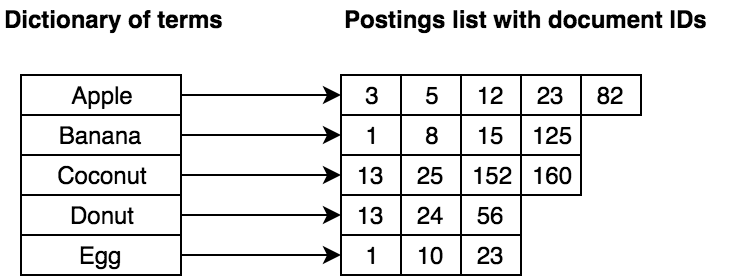
\includegraphics[width=0.7\linewidth]{images/chapter_2/inverted_index}
	\caption{An illustration of a simple inverted index}
	\label{fig:invertedindex}
\end{figure}



The inverted index consists of a dictionary and a postings list. The dictionary keeps track of the unique terms in the document collection, while the postings list keeps track of the document each term appears in. Other useful statistics associated terms are also stored in the index, common examples include term frequency (number of time a term, $t$ appears in a document,$d$), document frequency (number of documents containing term $t$) and the length of each document for normalisation operations. Figure \ref{fig:invertedindex} illustrates an  example of a minimal inverted index, with document IDs in the postings list. 

In a typical use case, a user attempts to represent their information needs in the form of a query, typically consisting of some number of terms. The system can perform a search in a number of ways. The most naive method combines exact term matching and boolean operations. The system first looks up each term in the dictionary, and then retrieves their postings list. The posting lists for the terms are combined and returned to the user. The combination is based on the user's specification of boolean operators, AND, OR, and NOT. These boolean operators correspond to various set operations. This method is known as boolean retrieval. It is one of the earliest form of retrieval methods, and is still available as a feature in some commercial search engines. 

\section{Relevance ranking}

Boolean retrieval is suitable for users that may know exactly what documents they are looking for, and the terms contained in those documents. However, this is not a typical search engine user's behaviour. A 2001 survey shows that less than five percent of web search engine user's use boolean operators during web search (Spink et at.,)\cite{spink2001searching}. A more typical user often begins with a vague idea of a topic, then searches in an iterative fashion. The typical process involves typing in a few terms, search, refine the query, and search again. This process repeats until the user either finds what they are looking for, or gives up from frustration and perhaps switches to another search engine. Boolean retrieval is unlikely to work well with this approach, because it creates a “feast or famine” like situation. Using boolean AND to join the terms in the query could result in too few documents being retrieved, while using boolean OR could result in too many to be useful to the user. The results presented by boolean retrieval are also not ordered to suit the user's information needs, instead ordered by the document ID stored internally in the index. This ordering is not useful to the typical user.

Ranked retrieval aims to solve this problem by sorting the results list based on their relevance to a user’s information need. However, deciding what the user's information needs are is a challenging problem. Usually only a limited amount of information about the user is known to the system. The problem facing information retrieval researchers in regards to satisfying the user's information need is essentially a problem of ``do what I mean, not what I say''. The system must model what is relevant to a user based on partial knowledge. Research in ranking aims to solve the problem of modelling relevance. Over the years several major models for computing relevance have been proposed and used, these will be covered in the next section.


\subsection{Paradigms in ranking}
\subsubsection{Vector Space Model}


One of the most prominent ranked retrieval models is the Vector Space Model, first proposed by Salton et al. \cite{Salton:1975:VSM:361219.361220} in the SMART information retrieval system. Under this model, each document in the collection is represented as a vector in a high dimensional vector space. Each unique term in the dictionary represents a new dimension in this vector space. The user's query is also viewed as a document, albeit with few terms, represented as a vector in the same vector space as the collection. 

Under this model, each document in the collection is represented by an $M$ dimensional, real valued vector, where $M$ is the total number of terms in the corpus. The value on each axis is determined by some term weighting scheme. The number of dimensions can be very large depending on the size of the corpus, thus each document vector is likely to be sparse. Most of the axis will be set at the origin due to a document only containing a small subset of all possible terms from the corpus. For this reason typically the vector space model only includes documents in the results list, where the query terms are contained. Another intuitive way to conceptualize the Vector Space Model is to view the vector space as a $M \times N$ matrix, where there are $M$ terms in the dictionary, and $N$ number of documents in the collection. 


The relevance of a document $d_1$, with respect to a user's query $q$, is determined based on similarity between the vector representation of the two, based on some distance function. Cosine distance is commonly used as the distance function. This is computed by the dot product between the two vectors as:

\begin{equation}
    sim(d_1,q) = \vec{v}(d_1).\vec{v}(q)
\end{equation}

The vector space model makes several assumptions about the query. Firstly, each term is assumed to be independent from other terms in the query. A document's relevance is based on the summation of contribution of each term inside the document, regardless of the order they may appear in. This is known as bag-of-words model. Secondly, terms are not equal. It is unlikely that every term in a user’s query would be equally relevant to the user’s information need. It is therefore necessary to weight the terms inside a document based on the likelihood of these terms being useful to the user's information needs. 


\subsubsection{Probabilistic ranking and language modelling}

A different paradigm to approach document ranking is by framing it as a probability problem. There are two major schools of thoughts within this paradigm; classical probability models prominent in early years of information retrieval, and the recent emergence of language modelling. 

Classical probabilistic retrieval was first proposed by Robertson and Spack-Jones (1976) along with the Binary Independence Model \cite{robertson1976relevance}. The key idea is that there are two classes of documents; either they are relevant to the user or not relevant. Various techniques are used to estimate the probability of a document falling into either of those categories, such as Naive Bayes, and the 2-Poisson model. \cite{robertson1994some}
While the performance of these early probabilistic models is not as good as a well tuned vector space model, the ideas behind this technique paved the foundation for the development of other approaches.

Ponte and Croft introduced the idea of language modelling in 1998\cite{ponte1998language}. This approach assumes that a document $d$ is an observation generated under a language model. In order to rank documents with regards to a query, a language model is first estimated for each document in the collection, and the document's relevance to a query is decided by the likelihood that the model which generated the document will also generate the query. Another way to think about this is the likelihood of getting the query by sampling random terms from the document, expressed as :

\begin{equation}
rel(d|q) = P(q|d) 
\end{equation}

The probability of generating a query from a document is computed from the product of the probability of generating each query term $t$, from document, $d$:

\begin{equation}
P(q|d) = \prod_{t \in q} P(t|d)
\end{equation}

The probability of $P(t|d)$ is estimated using the Maximum Likelihood Model, which can create a data sparseness problem. If a term is not in a document, then the probability of the document being relevant to the query drops to zero. This is mathematically correct, but unlikely to be helpul to the user. 

One approach to mitigate the sparsity issue is the use of background language model and smoothing techniques, which adjust the parameters in the Maximum Likelihood Model and assumes that a document is only a partial observation under the language model, estimating the hypothetical next term in the document from the collection. Effective choices include Direchlet smoothing and Jelinek-Mercer smoothing. Zhai and Croft(2004)\cite{zhai2004study} conducted a comprehensive study of various smoothing techniques and parameters to mitigate this issue, showing that more verbose queries, in general, are more sensitive to smoothing techniques, and combining multiple smoothing techniques are effective. 

Lavrenko and Croft \cite{lavrenko2017relevance} proposed an alternative approach to language modelling by combining classical probability models and language modelling. This technique provides an different solution to the sparsity problem, estimating terms relevant to the query based on the query alone. 

\subsection{Term weighing techniques}

In the vector space model, the placement of a term along a dimension is determined by some weighting factor. Various weighting schemes have been developed to weight terms based on modelling of user's intentions in order to rank documents that are more likely to be useful to the user highly. 

\subsubsection{TF.IDF}
An early weighting scheme is TF.IDF, proposed by Salton et al,.(1975) \cite{Salton:1975:VSM:361219.361220} alongside the original Vector Space Model.

Suppose term frequency,  $tf_{t,d}$ is the number of times a term $t$ in the user's query appears in a document, $d$. Intuitively, a document that has a higher $tf_{t,d}$ is more likely to be more relevant the query than a document with a low $tf_{t,d}$.

However, ranking the results naively by $tf$ becomes problematic. Firstly, term frequency alone does not model how well a document satisfies a user's information need, as it implies that all terms in the query are equally important, which is rarely the case. For example, in English language, terms like ``of'' and ``the'' are often connective terms that do not bear much semantic content.

Secondly, ranking by $tf$ alone assumes that relevance scales linearly with term frequency. Suppose a term $t$ appears in two documents, $d_1$ and $d_2$.  $d_1$ with a $tf_{t,d_1}=100$ is indeed likely more relevant than another document, $d_2$ with $tf_{t,d_2}=10$. Though it is unlikely to be 10 times more relevant compared to $d_2$. 

Inverse document frequency($idf$) was introduced to address this problem. The goal is to give rarer terms higher weight compared to common terms.

The inverse document frequency is computed as:

\begin{equation}
    idf_t = log \frac{N}{df_t}
\end{equation}

Where $N$ is the total number of documents in the collection.  The intuition is that if a query term appears in all of the documents, then it is not ``about'' any particular document. If a term appears in the query, and few documents from the collection, then it is highly likely that the document is relevant in relation to the term. 

Combining the two, the tf.idf ranking scheme becomes:

\begin{equation}
     tf.idf_t = tf_{t,d}. idf_t
\end{equation}

In practice, $tf$ is often normalized against the length of the document. This takes account of different document lengths. Intuitively, a longer document would be more likely to have a higher raw term count. Normalizing prevents biasing towards longer documents. This ranking scheme fits loosely with an observation based on Zipf's law\cite{li1992random}, which states that terms in a corpus would follow approximately an inverse proportional relation with it's own frequency. 

Though the idea behind TF.IDF is intuitive and straight forward to understand, it is a heuristics based method with little formal motivation. Developing an effective term weighting scheme to model a user's information need has been a problem of interest for decades in the information retrieval community. Much of this is due to ranking being an inherently difficult problem, it has been estimated that the mean number of terms in a web query is 2.4 \cite{spink2001searching}. Systems must infer user's intention from a relatively short query, which is a challenging task. Many variants of the basic TF.IDF weighting scheme have been developed in recent years, and this remains an active part of research.


\subsubsection{Okapi BM25}

Okapi BM25 is one of the TF.IDF like ranking function which combines elements of probabalistic retrieval with the vector space model. Originally developed along with the Okapi information retrieval system.It is a heuristics based method which combines the elements of BM11 and BM15 \cite{robertson1995okapi} BM25 defines relevance between a document,$d$, and a query, $q$ as:

\begin{equation}
    rsv(d,q) = \sum_{i=1}^{n} idf(q_i).\frac{f(q_i,D).(k_1 + 1)}{f(q_i,D) + k_1.(1-b+b.\frac{|D|}{avedl}}
\end{equation}

Where $q_i$ is the query term, $idf(q_i)$ is the inverse document frequency of $q_i$, designed to down weight terms that are common in the collection. $b$ and $k1$ are parameters,  $b$ controls the effect of document length (defined as the number of terms in the document) normalisation, the larger $b$ is, the more pronounced the effect of the length of the document compared to the average length of the document,  setting $b$  to 0 result in the length of the document being ignored completely. $k1$ determines the saturation of term frequency, controlling the degree of influence the term frequency of a single term add to the end ranking score. 

BM25 and it's many variants is widely considered to be state of the art in ranking function, and there has been little concrete evidence that any particular variant consistently outperforms the original benchmark in all situations (Trotman et al) \cite{trotman2014improvements}. It is often used as a baseline method in Information Retrieval research where other methods are compared to. 

In this thesis we use ATIRE's implementation of BM25 as one of the two baselines to measure the performance improvement of our replication of Nogueira \& Cho's query reformulation system. 


\section{Query Reformulation}
Users usually interact with a search engine in an iterative way, which involves browsing through the list of documents returned by the system, and rewriting the query until their information needs are satisfied. 

Automatic query reformulation is the sub field of information retrieval aimed at improving the user’s search experience by automatically reformulating queries for them. This is a broad area which loosely covers all the methods where the user’s query is edited or rewritten. 

Query reformulation can be approached either globally or locally. Global analysis covers techniques where the query is reformulated without considering the list of top documents returned from the initial round of a search. Well known global query reformulations techniques include using a thesaurus such as WordNet \cite{miller1995wordnet}, spelling correction and stemming. Local analysis is based on the assumption that the user’s initial query is at least reasonable representation of their information needs, and looking to improve the user’s query based on the initial set of returned documents. This is also known as relevance feedback. 

\subsection{Relevance feedback}

In classic, “true” relevance feedback the user would pass a query to the search engine,  receive the top results list, then provide human judgement on which documents are more relevant to their needs than others. A second round of search is performed with this additional information to find documents similar to those marked as relevant by the user. However, in most situations the user may not wish to provide such human judgement due to the added hassle. In these cases, pseudo relevance feedback is used. 

Pseudo relevance feedback, also known as blind relevance feedback is used without the need for user's relevance judgement  An assumption is made that if the ranking function is performing adequately, then the most relevant documents with regard to a query should be at the top of the results list. Another assumption is that the user’s query is a reasonable reflection of their information needs. If the initial query does not reflect the user’s true information needs, then it is likely that no amount of local analysis would achieve optimal results. 

There are many techniques to conduct relevance feedback. As relevance feedback is closely related to ranking, sharing the common goal of improving search effectiveness, many relevance feedback techniques are related to ranking models.  In this thesis we use ATIRE's implementation of pseudo relevance feedback as another baseline to compare the performance of our system with. (The other being raw ATIRE search with BM25 as the ranking function). 

\subsubsection{Rocchio's algorithm}

Rocchio’s algorithm is a classic relevance feedback method introduced alongside the Vector Space Model by Salton et al.\cite{Salton:1975:VSM:361219.361220}. It provides a theoretical framework for relevance feedback and pseudo relevance feedback by extension. 

The idea behind the algorithm is based on moving the query vector towards an unknown "optimal" query location in the high dimensional vector space. In order to maximize relevance the optimal query is moved towards the centroid of the set of relevant documents, and away from the set of non relevant documents. The details of the shift can be defined as :

\begin{equation} \label{eq:rocchio}
    \vec{q}_{opt} = \alpha \vec{q}_0 + \beta \frac{1}{|D_r|}  \sum_{\vec{d_j} \in D_r} \vec{d_j} - \gamma \frac{1}{|D_{nr}|}  \sum_{\vec{d_j} \in D_{nr}} \vec{d_j} 
\end{equation}

Where $\vec{q}_{opt}$ is the original query vector,  $D_r$ is the set of relevant documents, $D_{nr}$ is the set of non relevant documents. The aim is to shift towards the centroid of known relevant documents.  $\alpha$, $\beta$ and $\gamma$ are weights which dictate how much to shift the new query vector, which can be chosen based on the specific circumstance. For example, if the user provides ample information and tags many documents as relevant, then it is common practice to have a larger $\beta$ value, since the system has higher confidence level from the user's feedback. 

In the case of pseudo relevant feedback it is assumed that the top $k$ documents from the first round of search is relevant, and so we shift the optimal query towards the centroid of this set. In this scenario, the system does not have examples of non-relevant document, so the last part of the equation is dropped. An an alternative approach has been suggested by Robertson et al., \cite{robertson1999okapi}, who assumes that documents at the bottom of the list past some threshold is deemed non-relevant and can be used as the non-relevant set.


\subsubsection{ATIRE's pseudo relevance feedback}


ATIRE's pseudo relevance feedback combines the use of Rocchio's algorithm with KL-divergence as an indicator of potentially useful terms to add to a query. KL divergence is a metric used to measure the distance between two distributions, specifically, how frequencies in one distribution diverge from another,computed as:

\begin{equation}
D_{KL}{d||c)}= p(d).log\frac{p(d)}{p(c)}
\end{equation}


In the implementation ATIRE's pseudo relevance feedback, the top $k$ documents are grouped into a set, each unique term in the set is analysed. For each term, the term frequency in this retrieved set is $d$, and  term frequency in the rest of the collection is $c$.  On an intuitive level, this scheme identifies how much a term's frequency in the top $k$ document diverges from the expected, based on analysing the entire collection.  It is reasonable to assume terms that has a higher than expected frequency in this retrieved set compared to the rest of the collection are more ``about'' this set, and therefore likely to be relevant to the query which initially retrieved this set. 

The set of unique terms in the top $k$ documents are ranked from highest and lowest based on their computed KL-divergence score, and the top $m$ terms are added to the original query for pseudo relevance feedback using Rocchio's algorithm outlined in equation \ref{eq:rocchio}. In ATIRE's implementation of Rocchio's algorithm a design choice is made to ignores non-relevant documents because they cannot be identified with certainty, this equates to setting  $\gamma=0, \alpha=1, \beta=1$ in equation \ref{eq:rocchio},  thus the formula becomes:

\begin{equation} \label{eq:ATIRE_rocchio}
\vec{q}_{opt} = \vec{q}_0 +   \frac{1}{|D_r|}  \sum_{\vec{d_j} \in D_r} \vec{d_j}  
\end{equation}


 

\section{Evaluating Information Retrieval systems}

It is important to measure the performance of information retrieval systems in order compare two systems and attempt to make meaningful improvements, for we cannot improve what we cannot measure, various standard metrics in information retrieval exist for this task. 

\subsection{Metrics}


\subsubsection{Recall and precision}

Recall and precision are accuracy metrics that measure the performance of a system on a single query. 

For a given query,recall is defined as:

\begin{equation}
Recall = \frac{|retrieved\,documents \, and\,relevant\,documents|}{|relevant\,documents|}
\end{equation}

This is measurement of the number of documents found and known to be relevant, compared to the entire set of documents judged to be relevant (the ground truth).

This metric provides limited utility in practice, as it does not take into account the number of irrelevant documents in the retrieved set as long as the relevant documents are also in there somewhere. Consider an extreme example where the entire collection is retrieved, this is bound to result in a recall of 1 as any known relevant documents must be in this retrieved set, but the results list would be very noisy, frustrating the end user. 

Precision for a query is defined as:

\begin{equation}
Precision = \frac{|retrieved\,documents \, and\,relevant\,documents|}{|retrieved\,documents|}
\end{equation}

Precision measure the number of found documents that are relevant, compared to the number of documents retrieved by the query. 

A drawback of these accuracy metrics is that neither recall or precision take into account the positioning of the relevant result in the retrieved results list , simply optimizing for these metrics may lead in a noisy results list that provide little utility to the end user.


\subsubsection{Precision at k}

It can be reasonably assumed that users are unlikely to browse through a number of results returned, thus only the top $k$ results will be useful to the user. To model this idea,  precision at K (Precision@k) introduce the idea of a ranking threshold by only measuring the proportion of relevant documents in the top-K documents from the retrieved set. Let $T$ be the set of documents identified to be relevant. Precision@$k$ is computed as:


\begin{equation}
P@k =  \frac{\sum_{i=1}^{k} rel(i)}{k}
\end{equation}

\begin{equation}
rel(i)=
\begin{cases}
1, & \text{if } i\in T\  \\
0, & \text{otherwise}
\end{cases}
\end{equation}


The number of retrieved documents up to the cut off line, $k$ that are also known to be relevant is then reported as precision@k.

\subsubsection{Average Precision}
Average precision builds on the idea of precision@K and introduce the notion that placement of relevant documents in the results list is also important. For a given query, average precision is the mean of the precision scores after each relevant document is found, computed as:

\begin{equation}
	AP = \frac{\sum_{i}^{R} P@i}{R} 
\end{equation}

Where $R$ is the results list. 

In order to achieve a high average precision the system need to place relevant documents are the top of the results list, as well as push non-relevant results further down the list. 



\subsubsection{Mean average precision}
To compare the effectiveness between systems, Mean Average Precision(MAP) is often used, it provides a way to meaningfully compare two systems over a set of queries by taking the Average Precision of each query and taking the un-interpolated mean value as MAP. Let Q be the set of queries to be assessed, Mean Average Precision is computed as

\begin{equation}
	MAP =  \frac{\sum_{q \in Q} AP_q}{Q}
\end{equation}

For our experiments we compare MAP@40 of the reinforcement learning based system to baselines. The reason we chose to measure and report MAP@40 is that we are reproducing the framework of Noguiera \& Cho \cite{nogueira2017task} based on their written description, we wish to compare our reproduction of the system to the published results. 


%\section{State of Machine learning application in Information retrieval}
%
%Machine learning has been used in information retrieval
%
%
%Earlier applications include learning to rank using genetic algorithm and genetic programming.
%
%
%In recent year 
%
%
%
%
%* Learning to rank isn't suitable as a baseline here, because we want non learning components in the pipeline as the baseline, otherwise it's just a more complex learning system?
%
%We want to compare


\subsection{Standard datasets and human judgement}

It is important to be able to compare various information retrieval systems and algorithms in a fair, controlled fashion. MAP gives us a metric to compare systems over a set of queries. However, it is important that the systems are assessed in the same tasks to get an ``apples to apple'' comparison. For this reason, various standard datasets with human judgement are used. 

Ad-hoc retrieval datasets usually consists of a set of queries, sometimes referred to as topics or tasks, and a collection of documents to perform the search on. Human assessors read each document in the collection, and  provide judgement on which document is relevant to each query. Judgements can either be binary or graded,. In the case of binary judgement, a document is either considered relevant to a query or irrelevant.  In graded assessment, a score is provided on how much a document is about a query.  

Human assessment is typically very time consuming, as it could take many hours  to read and assess each document. For this reason datasets are usually judged as part of a collaborative effort, common sources of standard data sets are academic conferences and organizations such as TREC, INEX, CLEF and NCTIR.


\subsection{Significance testing}

When a set of queries are used to evaluate a system, it is usually not sufficient to only show improvement with a single metric such as MAP. We often need to know the proportion of queries that improved. Improving a single query by a lot and increasing all queries by small amounts would result in similar MAP scores, yet these two situations carry different implications. In this thesis we use Student's t-test as way to measure the significance in improvement between the deep reinforcement learning based system and baseline methods.


\section{Deep Reinforcement Learning}

As this thesis involves reproducing a deep reinforcement learning based query reformulation system, this section provides necessary background knowledge in deep reinforcement learning.

\subsection{Reinforcement learning as a paradigm}
Early development of reinforcement learning has followed a combination of two approaches. The first is natural learning inspired by the psychology of animal behaviour, the second is rooted in dynamic programming and value functions for optimal control. Bellman's equation being a fundamental framework for this approach \cite{bellman1966dynamic}. Through decades of development the modern field of reinforcement learning became as we know it today. 

Deep reinforcement learning is a combination of classical reinforcement learning algorithms with deep neural networks as function approximators, giving the agent added expressiveness and capability, but also increased instability. In recent years deep reinforcement learning has achieved outstanding results in control based tasks such as playing video games, such as ATARI games\cite{mnih2013playing} and Doom\cite{lample2017playing} , as well as board games such as Chess, Shogi and Go \cite{silver2017mastering} \cite{silver2016mastering}.

As a machine learning paradigm, reinforcement learning is different to supervised learning and unsupervised learning even though it shares similarity with these two paradigms. In supervised learning, an agent is exposed to a training set of examples with correct labels, with the goal of making predictions in the future against unseen test data. Unsupervised learning focuses on finding hidden structures in large amounts of data without labels, examples include dimensionality reduction techniques such as Principle Component Analysis, and clustering techniques such as K-Means clustering. Reinforcement learning shares some characteristics of these two paradigms, though fundamentally different from them. The problem of reinforcement learning involves an agent which learns from its own experience, with time delayed, sparse labels given to indicate its performance. While there is a goal to be achieved in the problem, the agent is not explicitly told which action to take (as it would in supervised learning), but instead needs to figure out what to do by trying them out. i.e., mapping situations to actions to maximize a scalar reward signal. 

\subsection{Key concepts in reinforcement learning}

\subsubsection{agent and environment}

A reinforcement learning problem consists of interactions between an agent and the environment. Figure \ref{fig:agent-environment} illustrates this interaction. The agent is the learner, which interacts with the environment at each time step, and learns from feedback signals received from the environment. The environment contains the task to be achieved or problem to be solved. Anything that the agent cannot directly influence by action output is considered to be part of the environment, this includes other agents in multi-agent environments. The environment provides the agent with an observation of the environment at each time step, which include the current state, and a reward. The observation is an important part of a reinforcement learning dynamic, specifically, the reward signal is crucial as it defines the agent's goal in a reinforcement learning problem. The task of defining a suitable reward function is a non-trivial issue. Ill defined reward functions can lead to unexpected and sometimes undesirable behaviours from the agent. 

\begin{figure}
	\centering
	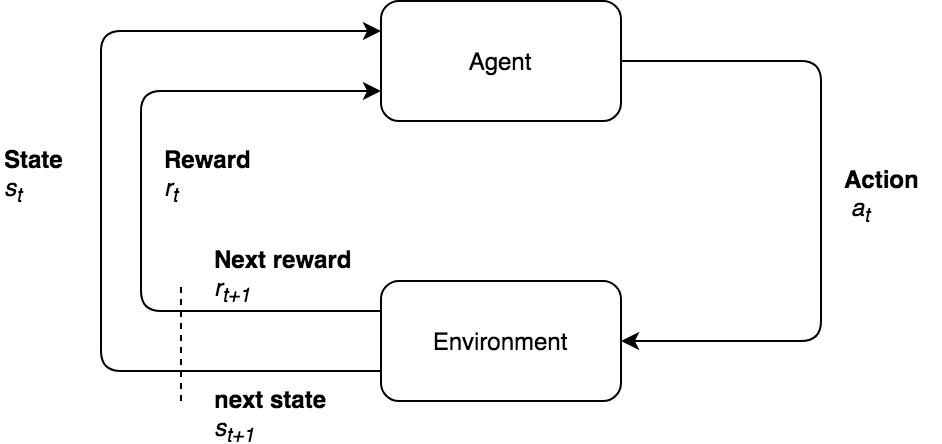
\includegraphics[width=0.7\linewidth]{images/chapter_2/agent-environment}
	\caption{The agent environment interface.}
	\label{fig:agent-environment}
\end{figure}



From a theoretical stand point, reinforcement learning problems can be formalized as special instances of Markov Decision Process, which can be solved by dynamic programming. In practice, however, dynamic programming is almost never a suitable method for solving reinforcement learning problems because it requires the agent to have a perfect model of the environment.



\subsubsection{The agent: policy, value function, and model }

Under the reinforcement learning framework, the agent's goal is to maximize the reward it receives; it achieves this by outputting actions into the environment according to some policy, $\pi$ . 

The policy is a mapping between the state, $s$, and an action, $a$, selected from all possible actions the agent may take, known as the action space.

Policy is a crucial part of the reinforcement learning agent, as it alone can determine the behaviour of the agent. A family of algorithms which iteratively optimize the policy directly towards the direction of more rewards is known as a policy gradient method, such as REINFORCE \cite{williams1992simple} and DDPG\cite{lillicrap2015continuous}. 

Additional to a policy, an agent may have a value function. This is the agents prediction to how good a given state is in the long term. The difference between rewards and value function is that the former is based on direct  and immediate response from the environment, which can be thought of as "ground truth" while the latter is based on an estimation generated from sequences of observations. Value based reinforcement learning revolves around the idea of gradually approximating the utility of every possible state, and move towards states that are higher in value. Notable examples of this includes Temporal Difference Learning\cite{tesauro1995temporal}  and Q-learning \cite{watkins1992q}.

Optionally, an agent might possess prior knowledge of the full dynamics of the environment and form a precise model of it. The agent can then exploit this prior information in planning based algorithms. In the case where the full dynamics of the environment is available to the agent, the reinforcement learning problem can be reduced to a dynamic programming problem. However, this is very rarely the case for reinforcement learning. Usually the problem consists of a black box environment where the agent has limited to no knowledge of the dynamics of the system, and must learn based on sampling a collection of past experiences. 

%\subsubsection{On-policy learning vs Off-policy learning}
%\todo{On vs off policy learning}


\subsubsection{Exploration vs exploitation}

As the agent's goal is to learn an optimal policy which maximizes cumulative reward over a time period based on partial information of the environment, whether the agent should behave in a greedy manner and take actions known to yield a good outcome, or taking more risk and explore unknown, and potentially suboptimal actions is a well known topic in the field of reinforcement learning. This is the notion of a exploration vs exploitation problem. In practice it is important to find a right balance between the two. As always exploiting short term gains leads to the agent converging to a local optimum which may be far from the global optimum, while only exploring would lead to the agent not converging on any policy.

\subsubsection{Common notation and conventions in reinforcement learning}

These are the essential components of a reinforcement learning problem, and we will use these notations from the remaining chapters of the thesis. 

\begin{itemize}
    \item $S$,the state space, this is the set of all possible states the environment can be. $s_t$ is the current state of the environment, as observed by the agent.
    \item $A$ the action space, the set of all possible actions that can be performed by the agent. $a_t$ is the action selected by the agent based on a given policy, at time $t$
    \item $\pi$ The policy, a mapping between state and action. Policy may be deterministic or stochastic, in the latter case, probabilities of taking an action is given.
    \item $r$, the reward, a scalar value given to the agent at each time step. The agent's goal is to maximize the cumulative rewards received from the environment. In a typical reinforcement learning problem a discount factor, $\gamma$, is used to discount the value of future rewards. Due to uncertainty, immediate rewards are usually weighted higher than rewards achievable in the future. 
\end{itemize}




\subsection{Policy Gradient methods}


Policy gradient methods are a class of reinforcement learning algorithms which perform search directly in the policy space for a policy which leads to higher cumulative reward. This is fundamentally different to the approach of value based methods, where the agent predicts the desirability to be in a given state, and choose actions accordingly. Instead, policy gradient methods learn a parametrized policy, where a parameter vector $\theta$ dictates the agent's action when presented with a state under such policy. This can be expressed as:

\begin{equation}
    \pi(a|s,\theta) 
\end{equation}

The policy $\pi$ is driven by the parameters, $\theta$, often notated as $\pi_{\theta}$. The agent's goal is to find the values in the parameter vector which leads to optimal outcomes, based on the gradient of some performance measure, $J(\theta)$ with regard to the parameters themselves. The update process can be formalized as: 

\begin{equation}
    \theta_{t+1} = \theta_t +  \widehat{\alpha \nabla J(\theta_t)}
\end{equation}

Where $\widehat{\alpha \nabla J(\theta_t)}$ is an approximation of the gradient of performance measure with respect of the parameters, $\theta$. The gradient is estimated from a collection of past experience known as trajectories. The trajectory consists of a collection of historic information, specifically, a mapping between state, action taken, immediate reward received from taking such action, and the state of the environment after taking the action.

Theoretically, policy gradient methods do not require a value function. However, in practice a state-value function is often used to speed up learning and reduce variance. If the state value function is a learnt function, this method becomes an actor-critic method. Well known algorithms in this family include REINFORCE, DDPG\cite{lillicrap2015continuous} and A3C\cite{mnih2016asynchronous}. We use REINFORCE as the core reinforcement learning mechanism for the query reformulation agent in our experiments.


\subsubsection{REINFORCE algorithm} 

REINFORCE is a policy gradient method proposed by William et al \cite{williams1992simple}. It is a Monte-Carlo method, meaning that the agent learns from exploring experience trajectories without building an explicit model of the environment. 
This algorithm is expressed in the following pseudo code:

\begin{algorithm}[H]
	\caption{REINFORCE algorithm}\label{alg:REINFORCE}
	\begin{algorithmic}[1]
		\Procedure{REINFORCE}{}  
		\State $\theta\gets initialize$
		\For {generate trajectory \{ ${s_1,a_1,r_2...s_{T-1},a_{T-1},r_{T}}$\}  by following $\pi_{\theta}$}
		\For {$t=1$ to $T-1$}
		\State estimate the return $G_t$ 
%		\Comment{current reward and discounted future returns}
		\State $\theta \gets \theta + \alpha \gamma^tG_t \nabla\log \pi(A_t|S_t,\theta)$
		\EndFor
		\EndFor
		\State \textbf{return} $\theta$  
		\EndProcedure
	\end{algorithmic}
\end{algorithm}


Where $\alpha$ is the learning rate, $\gamma^{t}$ is a discount factor for time step $t$, and $G_t$ is the return at the current time step, defined recursively by the sum of the immediate reward,$r$ at the current time step, and the discounted return of future states reachable from the current state.  The intuitive interpretation of the algorithm is to let an agent collect experience in an environment by following a parametrised policy, then update the parameters based on the outcome of doing so. 



\section{Neural Networks related topics}

In this section we provide background knowledge in topics related to neural networks. 

\subsection{Perceptron}

The base unit of a neural network is a perceptron, commonly referred to as neurons or nodes in literature. It is a linear classifier model loosely inspired by the structure biological neurons, first invented by Rosenblatt in 1958. \cite{rosenblatt1958perceptron}

We illustrate the working on a perceptron on a simple problem in figure \ref{fig:perceptron}, this model taking in three input values, $x_1$, $x_2$ and $x_3$, combine it with three learned weights and a bias value, producing a single output.

\begin{figure}[H]
	\centering
	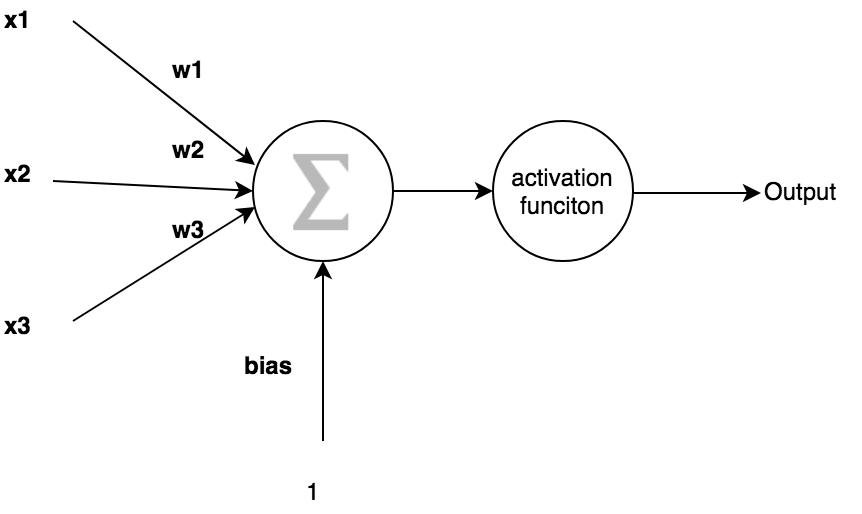
\includegraphics[width=0.7\linewidth]{images/chapter_2/Perceptron}
	\caption{An illustration of a perceptron}
	\label{fig:perceptron}
\end{figure}


From a linear algebra perspective, this model takes the dot product of the input vector $\mathbf{x}$ and a weight vector, $\mathbf{w}$ , with a bias value added to it, and passing the result to an activation function, $f$. In the classic perceptron, a step function is used as the activation function, this is expressed as:

\begin{equation}
	f(x) =
	\begin{cases}
	1 & \text{if $\mathbf{x} . \mathbf{w} + b > 0$},   \\
	0 & \text{otherwise}
	\end{cases}
\end{equation}

A single neuron with a step-function can only learn linearly separable patterns, which has limited practical utility. However, by combining multiple neurons with non-linear activation functions, more complex problems can be solved.


\subsection{Feed forward Neural Networks}

A feed forward neural network, commonly referred to as a fully connected neural network is neural model with multiple neurons, and at least one hidden layer. A hidden layer refers to a layer of neurons between the input and output layer, taking the output from previous layer as the input to the current layer. In a fully connected neural network, every neuron in the previous layer is connected to every available neuron in the next layer. In figure \ref{fig:feedforward} we provide a simple illustration of a fully connected neural network with a single hidden layer,  with 3 neurons in each layer.


\begin{figure}[H]
	\centering
	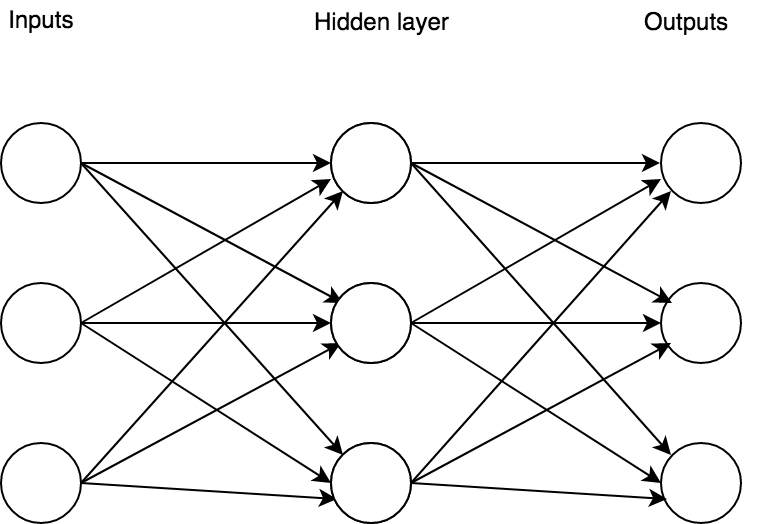
\includegraphics[width=0.7\linewidth]{images/chapter_2/feed_forward}
	\caption{A small fully connected neural network}
	\label{fig:feedforward}
\end{figure}


Mathematically, a layer of neurons can be viewed as a matrix of weights, the output of the layer being the result of taking the dot product of an input vector and this weight matrix, with a vector of bias values added to the result, passing through an activation function. Unlike the perceptron, each neuron in a feed forward neural network uses a non-linear activation function, common choices include, but not limited to sigmoid, softmax, and hyperbolic tangent. This gives the notion of gradient, allowing errors to be back-propagated in training using gradient descent, where the weights of the neurons responsible for producing the error gets updated in the direction of less error.



In a fully connected neural network model, each neuron in every layer is connected to all neurons in the previous layer. In principle, this would create a general purpose neural network capable of learning any function. The universal function approximation theorem states that a single layer of neurons with a finite number of neurons is capable of learning any arbitrary function.\cite{cybenko1989approximation}. This claim makes neural network sound incredibly attractive. However, the number of neurons required would make the network infeasibly large, computation expensive beyond practicality, and it may fail to generalize. 

Having more than one layer allows for more efficient learning with fewer neurons. For this reason, feed forward neural network often has more than one hidden layer, this is referred to as deep neural network, or deep learning.  The exact number of neurons, as well as the number of layers required to solve a problem depends on the task, and the size of the problem. This remains an open problem with little formal motivation. Much of these still rely on human intuition and trial-and-error, making deep learning a fascinating yet challenge field.

The fully connected architecture of a feed forward neural network makes this model computationally expensive and difficult to tune, for these reasons it is less common to train a fully connected deep model on a task from scratch using raw inputs for application purposes. A much more common usage of a fully connected deep network is to perform classification on features extract in earlier layers of a neural model, using convolutional layers.


\subsection{Convolutional Neural Networks}

Convolutional Neural Network (CNN) is a deep neural network architecture popularised by LeCun et al \cite{lecun1989backpropagation}.  First used for handwriting recognition, it became widely popular as the state of the art in deep learning. It has shown impressive results in tasks such as image processing, and used extensively in both industry and academic research, well known applications including facial recognition and the development of autonomous vehicles.

The key feature of CNN architecture is the introduction of convolution layers to a neural model. In such layer, kernels are used for local feature extraction. This kernel is also commonly referred to as a filter. It is represented as a matrix of weights, the idea being rooted in image processing and computer vision, inspired by the likes of the Sobel Filter.

 Instead of attaching every dimension in an input vector to the network like a fully connected neural network, in convolution layers features are computed by moving the kernel across the input according to a predefined stride. At each step, each element in the filter is multiplied with each input value the filter is currently overlapping, these elements are then summed together,producing a single value as the feature. As the filter moves through the input, a feature map is formed.
 
%  \todo{Image of CNN filter processing input}
 
 This design allows the neurons in the network to share weights, based on the assumption that there is local spatial correlation in the input. CNN introduces the notion of partial connectivity to the network, learning local features in earlier layers before combining the features in later layers.

The features generated through this convolution process are then passed through an activation function. The most common activation function following a convolution layer is ReLU (Rectified Linear Unit) defined as:

\begin{equation}
	ReLU(x) = Max(x,0)
\end{equation}




\subsubsection{Pooling}
Another important component that is often used in Convolutional neural network is pooling. This is a method for downsamping the output of the previous layer. The most common used approach is max pooling, where the max value of each region in the feature map is kept, and the rest is discarded. \todo{Expand?}


\subsubsection{Classification}




\subsection{Neural Language embedding schemes}

Terms in the English language holds semantic meaning that can easily be interpreted by a human reader, but not to a computer. In order to work with these terms they must be converted to a feature representation that is appropriate for machine processing. Given that terms are discrete features, the most traditional way is to represent text as sparse one-hot vectors of $k$ dimensions, where $k$ is the size of the corpus. To represent a term, the corresponding dimension in the one hot vector would be a one, and all other dimensions would be zero. The result of this is a sparse, high dimensional vector. 

Word embedding schemes are a class of methods used to map terms normally represented in such high dimensional space to a dense, low dimensional space as vectors. This has several benefits. Firstly, reducing the number of dimensions make computation more efficient. Training samples consisting of dense, lower dimensional representations are more suited for deep learning based models compared to the spare, high dimensional one hot vectors. These dense features are more likely to be captured by convolutional neural networks. Secondly, this mapping capture important relationships between these entities and place the vector representation in close proximity from each other. A popular example often used to illustrate this point is that the vector "king" subtracted by ``man'' gives us ``queen'' in a well trained model.
 
Early Word embedding schemes can be traced back to the Vector Space Model outlined in earlier parts of this chapter, and work has been ongoing for the past several decades. The development is largely motivated by the interest to capture semantic relationships between terms as well as the reduction of dimensionality.  

Recent development in deep learning saw the rise of neural network based word embedding schemes, such as GloVe \cite{pennington2014glove},fastText \cite{bojanowski2017enriching}, and Word2Vec\cite{mikolov2013distributed}. In our experiments we use Word2Vec embedding scheme, further details will be provided in chapter \ref{chap:new_ideas}. 


\section{Chapter summary}

In this chapter we provide background on various topics in information retrieval, reinforcement learning and neural networks. 

Finally we finish with an overview of state of the art in current query reformulation system rooted in deep learning. In the next chapter we describe our framework and the implementation of our system.